\documentclass[10pt,a4paper]{article}
\usepackage[margin=1.8cm]{geometry}
\usepackage{fontspec,xeCJK,amsmath,amssymb,booktabs,graphicx,hyperref}
\setCJKmainfont{Songti SC}
\setlength{\parindent}{0pt}\setlength{\parskip}{5pt}
\hypersetup{colorlinks=true,urlcolor=blue}
\title{Lean AM 梯度可靠性：后续实验与失败边界}
\author{可复核开发实验记录}\date{2026年10月25日}
\begin{document}\maketitle\vspace{-1em}
\textbf{结论：尚未得到稳定超越原始 AM 的新 HJBI 算法。}
有限步代价值保护在两个任务上均失败。将终点 critic 的 ReLU 换为 SiLU，
六关节任务平均代价降低 2.60\%，但仅 2/3 seed 胜出；导航恶化 3.64\%。
这是一条梯度估计的局部线索，不能当作鲁棒算法有效性的证明。
\section*{1. 完整结果与公平性}
两个原有自然任务，沿用 seed 18001--18003、原始标量数据及环境配置。
所有 actor 均使用 lean adjoint 与 Adam，1000 次更新，最终固定 checkpoint，
4096 条固定评估轨迹。没有刻意注入梯度误差，没有新增真实终点观测。
共 7 组方法、2 个任务、3 个 seed，即 42 次训练；不包含复现和诊断重放。
\begin{center}\small
\begin{tabular}{lrrrr}\toprule
方法 & 导航代价 & 相对改善 & 六关节代价 & 相对改善\\\midrule
Original lean AM + Adam & 19.4677 & -0.00\% & 10.9735 & -0.00\% \\
AM + Adam (2x rollouts) & 19.4139 & +0.28\% & 10.8092 & +1.50\% \\
AM + nominal value guard & 19.6124 & -0.74\% & 11.0959 & -1.12\% \\
AM + robust value guard & 19.6422 & -0.90\% & 11.2098 & -2.15\% \\
AM + RBF critic & 19.3162 & +0.78\% & 13.0453 & -18.88\% \\
AM + residual correction & 19.3649 & +0.53\% & 11.0179 & -0.40\% \\
AM + SiLU critic & 20.1755 & -3.64\% & 10.6884 & +2.60\% \\
\bottomrule\end{tabular}\end{center}
改善为相对原始 AM 的代价降幅；负数代表变差。
value guard 使用 64000 条训练 rollout 加 64000 条模型内检查 rollout；
AM (2x) 用 128000 条训练 rollout。其余每组 64000 条 actor 训练 rollout。
额外模型计算不是免费的；相同 rollout 数也不等于相同计算量。

\textbf{SiLU 六关节逐 seed：}
\begin{center}\begin{tabular}{rrrr}\toprule
seed & 原始 AM & SiLU 标签 & 相对改善\\\midrule
18001 & 10.3925 & 10.2569 & +1.30\% \\
18002 & 10.9999 & 11.3576 & -3.25\% \\
18003 & 11.5282 & 10.4507 & +9.35\% \\
\bottomrule\end{tabular}\end{center}
平均改善主要来自 18003。配对代价差为 $-0.2851$，描述性 95\% t 区间
$[-2.0966,1.5264]$，包含零。复用了开发 seed，且依次探索了多个分支，
这不是独立确认，也不能把此区间当作选择校正后的显著性结论。
没有新候选通过预设的至少 1\% 改善且 3/3 胜出的推进条件，没有扩展新 seed。
\newpage
\section*{2. 实际实现的方案，不是新的控制目标}
固定真实目标与 lean 标签：
\[
J_g(\theta)=\mathbb E\!\left[\sum_{k=0}^{K-1}\Delta t
\left(\tfrac12\|u_\theta(X_k,t_k)\|^2+\ell(X_k,t_k)\right)+g(X_K)\right],
\]
\[
\tilde a_K=\nabla\hat g(X_K),\quad
\tilde a_k=F^\top\tilde a_{k+1}+\Delta t\nabla\ell_k,\quad
y_k=-S^\top\tilde a_{k+1},\quad
L_{\rm AM}=\tfrac12\mathbb E\sum_k\Delta t\|u_\theta-y_k\|^2.
\]
轨迹与标签 stop-gradient；没有 $D_xu$。Adam 学习率 .002、梯度裁剪 5。
lean matching 梯度不被等同为真实 $\nabla_\theta J_g$。

\textbf{A. 有限步代价值保护。}
每 20 个原始 AM+Adam 更新产生参数提议 $d$，在同一批 Brownian 噪声上
对 $\alpha\in\{0,1/4,1/2,1\}$ 各执行 320 条模型 rollout。
\[
\alpha_*\in\arg\min_\alpha\max_{w\in W}
\sum_mw_m\big[\widehat J_{g_m}(\theta+\alpha d)-\widehat J_{g_m}(\theta)\big].
\]
$W$ 沿用全局 critic 混合权重的单纯形、KL 半径 .3 和原始 noisy validation
MSE 约束。同一个 $w$ 比较候选与基准策略；普通检查固定均匀权重。
只插值参数，Adam 动量继续累计所有提议 minibatch。

因为零步在候选集中，选中步的\emph{经验候选集最坏差值}不大于零。
这不意味着真实代价下降：需要真实 $g$ 被集合覆盖，并控制 Monte Carlo 误差。
若固定估计满足 $|\hat g-g|\leq\epsilon$（覆盖两策略终点分布），则
$|\Delta J_{\hat g}-\Delta J_g|\leq2\epsilon$；本实验没有这样的覆盖保证。
数值检查可以避开直接求导，但不能凭空消除共同模型偏差。

\textbf{B. 数据锚定的梯度估计。}
RBF 核岭回归拟合原始标量 $y$，或原网络残差 $y-\bar g(x)$：
\[
\alpha=(K+\lambda I)^{-1}(y-\bar y),\qquad
\hat g_{\rm RBF}(x)=\bar y+k(x,X)\alpha.
\]
输入按训练数据标准化，长度尺度 $\{.5,1,2,4\}$ 与岭系数
$\{.001,.01,.1,1,10\}$ 只由原始 noisy validation MSE 选择。
这是显式平滑先验，不是梯度误差已校准的后验；六关节直接 RBF 反而显著变差。

\textbf{C. 固定的 SiLU 对照。}
只替换两层激活函数，保持数据、线性层初始化、参数量、bootstrap/minibatch
随机序列、critic 更新预算及验证选 checkpoint 规则不变。
actor 算法完全不变。这是终点标签估计的对照，不能声称提出了新 HJBI 方程。

\textbf{为什么保护失败？}
独立真实代价诊断抽查每五个 block：六关节 robust guard 修改了 17 个提议，
其中 11 个在独立样本上实际有益，只有 6 个有害。
该统计是有限样本符号检查，不是因果判定；它展示了有用步骤被缩短的问题。
\newpage
\section*{3. 梯度链路诊断与可复核性}
在完全相同的原始 AM actor（500/1000 步）上，使用每次 1024 条新轨迹，
比较不同终点估计。共同历史 Adam 的一阶、二阶动量也固定。
真实终点值与梯度仅用于这些训练后的诊断。
\begin{center}\small\begin{tabular}{lrr}\toprule
六关节共同路径上的指标 & 原始 ReLU & SiLU\\\midrule
代价值相对 RMS 误差 & 0.2149 & 0.2145 \\
终点梯度相对误差 & 0.3283 & 0.2353 \\
lean actor 梯度相对误差 & 0.7452 & 0.5737 \\
lean actor 梯度余弦 & 0.6418 & 0.8181 \\
共同历史 Adam 步向量相对误差 & 0.3065 & 0.2459 \\
共同历史 Adam 步向量余弦 & 0.9484 & 0.9366 \\
\bottomrule\end{tabular}\end{center}
代价值相对误差几乎相同，但终点梯度误差下降约 28.3\%，lean actor 梯度
相对误差下降约 23.0\%。这是与 motivation 一致的证据线索。
然而相对值误差约 21\% 并非近乎精确；共同历史 Adam 步向量的余弦还略有下降。
不应将这组指标包装成完整因果证明或稳定性能保证。
\begin{center}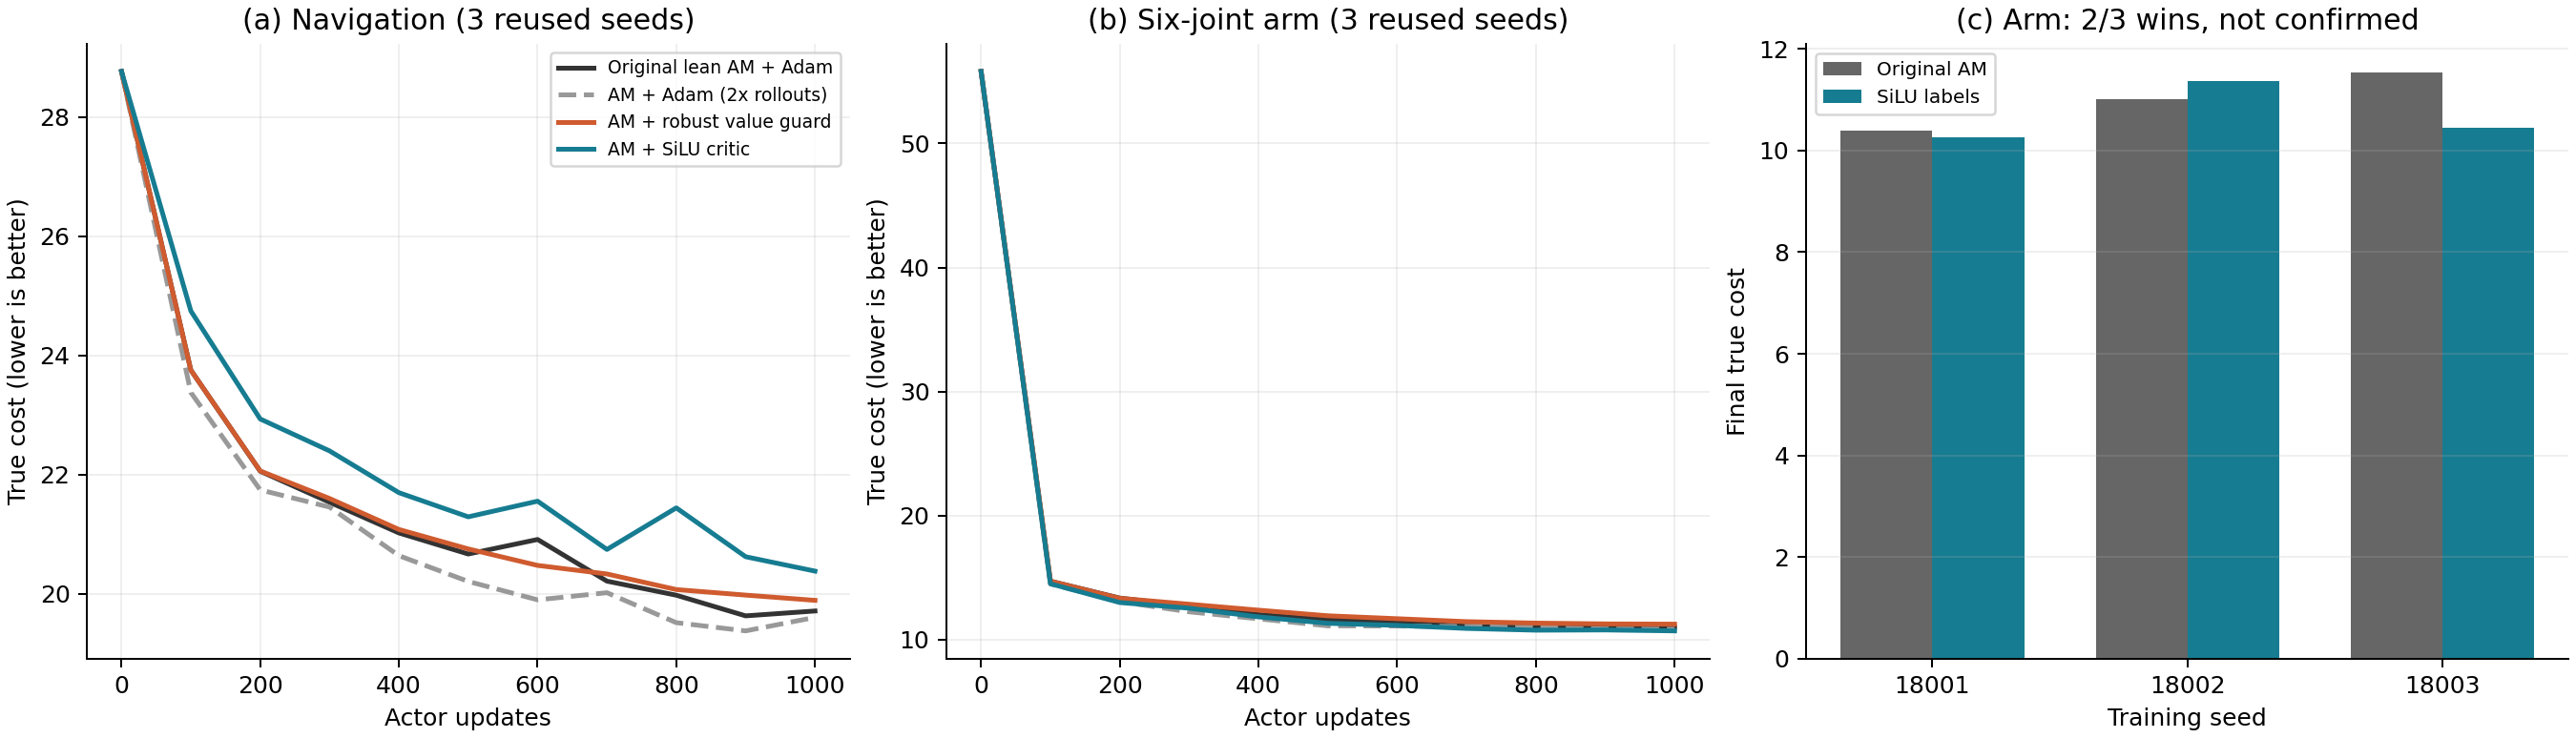
\includegraphics[width=\linewidth]{figures/followup_results.png}\end{center}
\textbf{审计与复现。}
原始 42 个输入文件及原训练源文件保持不变；六个原始 AM 重跑的最终指标逐项完全一致。
guard 的 1200 项凸支持函数用独立对偶上界复核，其中 6 项未通过
$2\times10^{-5}$ 的严格间隙阈值，最大归一化上界间隙为 0.001082；
这些告警保留，不能写成全部数值检查通过。
但 300 个最终选中步均通过候选集内经验代价不增加的上界检查。
更新检查禁止真实标签调用和 full-adjoint。
notebook 展示全部结果与代码，并从新 actor 完整重放一个 robust guard 和一个 SiLU 实验，
各 1000 次更新；结果与原始记录对齐。没有只从保存的终值拼接结果。

\textbf{结论边界。}
当前能保留的是：六关节中\emph{值误差近似相同、梯度更准确、平均性能更好}的候选线索。
没有证实梯度不确定性惩罚有效，没有独立确认，也没有稳定跨任务优于 AM 的新算法。
停止继续扩展这批开发实验，保留失败结果。
\small

参考：\href{https://arxiv.org/html/2409.08861v5}{Adjoint Matching, Sec. 5.2}；
\href{https://arxiv.org/html/2507.15082v1}{Robust Control with Gradient Uncertainty}。
本文检查和估计器对照是探索性实现，不是上述论文的实验结论。
\end{document}
